\clearpage
\chapter{\textbf{Grundlagen}}\label{grundlagen}
%\addtocontents{toc}{\vspace{0.8cm}}

\section{Machine Learning}\label{unterkapitel}
\addtocontents{toc}{\vspace{0.8cm}}

Grundsätzlich beschreibt Machine Learning das Entwickeln mathematischer Modelle zur statistischen Auswertung
von Daten. Dabei wird dem Modell anhand von Daten zu einem bestimmten Sachverhalt beigebracht, in einem 
Datenset Schemata zu erkennen, womit sich eine Erwartung über die Umstände des Datensets treffen lässt.
Beispielsweise könnte ein solches Model aus einem Datenset mit der aktuellen Jahreszeit, Uhrzeit und 
Position der Sonne am Himmel trainiert werden, sodass es auch schließlich in einem anderen Datenset 
aus Jahreszeit und Position der Sonne Rückschlüsse auf die Uhrzeit treffen kann.\\
Als Vorbild für diesen ,,Lernvorgang'' dient das menschliche Gehirn, welches ebenfalls versucht zwischen 
bestimmten Input-Parametern wie z.B. der Form und Farbe eines Gegenstandes eine Beziehung herzustellen,
um das beobachtete Objekt in Zukunft schneller kategorisieren zu können.\\
Da eine Vielzahl von effektiven Machine Learning Algorithmen existiert, ist es essenziell, sich mit den
Stärken und Schwächen einzelner Herangehensweisen zu befassen.\newpage

Im Wesentlichen kann Machine Learning in zwei Unterkategorien unterteilt werden:
\begin{itemize}
    \item \textit{Supervised Learning} 
    \item \textit{Unsupervised Learning}
\end{itemize}
\textit{Supervised Learning} bedeutet zwischen bestimmten Feldern eines Datensets eine Beziehung
zu einem sog. Label herzustellen, welches als eine Art Ergebnis aus den Eingabewerten gesehen 
werden kann. Ein so traniertes Model kann dann neue, ihm vorher unbekannte Datensets, mit einem 
Label versehen - etwa wie in dem o.g. Beispiel wo Jahreszeit und Sonnenposition die Eingabewerte 
und die Uhrzeit das Label darstellen. Der Begriff ,,\textit{supervised}'' ergibt sich daraus, dass 
das Datenset, mit dem das Model traniert wird, diese Labels gegeben 
hat, sodass das Modell sich bei jedem Schritt des Lernvorgangs selbst korrigieren kann, falls 
eine Fehleinschätzung getroffen wurde.
Bei einer sog. ,,\textit{Klassifizierung}'' sind diese Labels fest vorgegeben, während sie in der 
,,\textit{Regression}'' kontinuierlicher Natur sind.\newline\newline
Beim ,,\textit{Unsupervised Learning}'' versucht das Modell ohne Referenz zu einem bestimmten 
Label, Zusammenhänge zwischen bestimmten Feldern des Datensets herzustellen. Solche Modelle 
arbeiten vorrangig mit ,,\textit{Clustering}'' und ,,\textit{Dimensionality Reduction}''.\\
,,\textit{Clustering}''-Algorithmen versuchen ein Datenset in kleinere Bereiche einzuteilen und
so aus den Feldern des Datensets bestimmte Abhängigkeiten abzuleiten.
\begin{figure}[h]
    \centering
    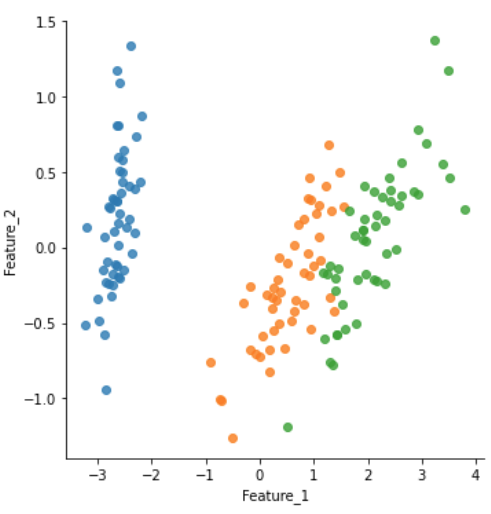
\includegraphics[width=8.0cm]{./pic/Clustering_Beispiel.png}
    \caption{Beispiel für Clustering}
    \label{fig:Clustering_Beispiel}
\end{figure}

Bei der ,,\textit{Dimensionality Reduction}'' versucht der Algorithmus das Datenset in einer 
Dimensionalität, also seiner Anzahl an Feldern, zu reduzieren. Es wird also die Frage gestellt, 
ob das bestehende Datenset auch mit weniger Feldern Abhängigkeiten feststellen lässt. Dieser 
Schritt wird vorallem für Modelle benutzt, die sensibel gegenüber hoher Dimensionalitäten sind, 
sodass das Datenset vor dem Training in seiner Dimensionalität heruntergebrochen werden kann.

\begin{align}
(p_i * p_j)(n) & =  \sum_{k \in \mathbb{D}} p_i(k) \cdot p_j(n - k) \\
p_{total} & =  p_0 \ast p_1 \ast \ldots p_{n-1}; \forall n
\end{align}

% Formel
Hier ist nur eine einfache Formel mit der \texttt{equation}-Umgebung für die Minkowski Metrik:
\begin{equation}\label{Minkowski}
D\left(X,Y\right)=\left(\sum_{i=1}^n |x_i-y_i|^p\right)^{1/p}\\
\end{equation}

Wie in Gleichung \ref{Minkowski} zu erkennen ist, ergibt sich die L2-Norm (Euklidische Distanz), wenn man den Exponenten $p = 2$ wählt.

Support Vector Machines \cite{Haykin99} nutzen die Euklidische Distanz (oder äquivalent) das Skalarprodukt.
%% Zwei Abbildungen, die zusammen gehören

%\begin{figure}
%        \centering
%        \begin{minipage}[c]{0.45\textwidth}
%                \includegraphics[height=6.5cm]{pic/dateiname1.png}
%        \end{minipage}
%        \begin{minipage}[c]{0.45\textwidth}
%                \includegraphics[height=6.5cm]{pic/dateiname2.png}
%        \end{minipage}
%        \caption{Zwei Abbildungen}\label{fig:zwei_abb}
%\end{figure}
